% ************************************************************************** %
% Copyright (C)  2016  Philipp Hacker.																			 %
% Permission is granted to copy, distribute and/or modify this document			 %
% under the terms of the GNU Free Documentation License, Version 1.3				 %
% or any later version published by the Free Software Foundation;						 %
% with no Invariant Sections, no Front-Cover Texts, and no Back-Cover Texts. %
% The lincense itself can be found at <https://www.gnu.org/licenses>.        % 
% ************************************************************************** %

%LICENSE:
%CC BY-NC-SA 3.0 (http://creativecommons.org/licenses/by-nc-sa/3.0/)

% Masters Thesis 
% LaTeX Template
% Version 2.3 (25/3/16)

% This template has been downloaded from:
% http://www.LaTeXTemplates.com

% Version 2.x major modifications by:
% Vel (vel@latextemplates.com)

% This template is based on a template by:
% Steve Gunn (http://users.ecs.soton.ac.uk/srg/
%						  softwaretools/document/templates/)
% Sunil Patel (http://www.sunilpatel.co.uk/thesis-template/)

% ************************************************************************** %
% ************************************************************************** %

% START OF TEX
\documentclass[
	10pt,
	twoside,
	chapterinoneline,
	onehalfspacing, % alternatives: onehalfspacing or doublespacing
	nolistspacing, % If the document is onehalfspacing or doublespacing,
								 % uncomment this to set spacing in lists to single
	%liststotoc, % Uncomment to add the list of figures/tables/etc to toc
	%toctotoc, % Uncomment to add the main table of contents to the toc
	parskip, % Uncomment to add space between paragraphs
	headsepline, % Uncomment to get a line under the header
	english,
]{MastersDoctoralThesis} % The class file specifying the document structure

% ************************************************************************** %
% CORE USEPACKAGE HERE
\usepackage{lmodern}
\usepackage[utf8]{inputenc} % Required for inputting international characters
\usepackage[T1]{fontenc} % Output font encoding for international characters
\usepackage[autostyle=true]{csquotes}
% Required to generate language-dependent quotes in the bibliography
%\usepackage[backend=bibtex,style=authoryear,natbib=true]{biblatex}
\usepackage[backend=bibtex,natbib=true]{biblatex}
% Use the bibtex backend with the authoryear citation style
\addbibresource{master_thesis.bib} % The filename of the bibliography
% ************************************************************************** %

% ************************************************************************** %
% MARGIN
\geometry{%
	% showframe, % show how the type block is set on the page
	paper=a4paper, % Change to letterpaper for US letter
	inner=2cm, % Inner margin
	outer=3.0cm, % Outer margin
	bindingoffset=1.5cm, % Binding offset
	top=1.5cm, % Top margin
	bottom=1.5cm } % Bottom margin
% ************************************************************************** %

% ************************************************************************** %
% THESIS INFORMATION
\date{\today} 
\thesistitle{Kinetic\ effects\ in\ RF\ discharges}
% Your thesis title, this is used in the title and abstract
\supervisor{Prof.\ Dr.\ Ralf\ Schneider}
% Your supervisor's name, this is used in the title page
\examiner{Prof.\ Dr.\ Jürgen\ Meichsner}
% Your examiner's name, this is not currently used anywhere in the template
\degree{Master\ of\ Science\ -\ Physics}
% Your degree name, this is used in the title page and abstract
\author{Philipp\ Hacker}
% Your name, this is used in the title page and abstract
\addresses{Karl-Liebknecht-Ring\ 13,\ 17491\ Greifswald}
% Your address, this is not currently used anywhere in the template
\subject{Physics}
% Your subject area, this is not currently used anywhere in the template
\keywords{plasma,\ discharge,\ kinetic,\ effect,\ physics,\ master}
\university{\href{https://www.uni-greifswald.de/en/}%
					 {Ernst-Moritz-Arndt\ University\ of\ Greifswald}}
% Your university's name and URL, this is used in the title page and abstract
\department{\href{https://physik.uni-greifswald.de/en/}%
					 {Institute\ of\ Physics}}
% Your department's name and URL, this is used in the title page and abstract
\group{\href{https://physik.uni-greifswald.de/ag-schneider/}%
			{Computational\ Sciences}}
% Your research group's name and URL, this is used in the title page
\faculty{\href{https://mnf.uni-greifswald.de/en/faculty/}%
				{Faculty\ of\ Mathematics\ and\ Natural\ Sciences}}
% Your faculty's name and URL, this is used in the title page and abstract
% ************************************************************************** %

\hypersetup{pdftitle=\ttitle} % Set the PDF's title to your title
\hypersetup{pdfauthor=\authorname} % Set the PDF's author to your name
\hypersetup{pdfkeywords=\keywordnames} % Set the PDF's keywords to your keywords

% ************************************************************************** %
% PACKAGES
\usepackage{amsmath,mathtools}
\usepackage{amssymb}
\usepackage{upgreek}
\usepackage{esint}
\usepackage{graphicx}
\usepackage{ziffer}
\usepackage{float}
\usepackage{wrapfig}
\usepackage{csquotes}
\usepackage{sectsty}
\usepackage{nomencl}
\usepackage{svg}
% ************************************************************************** %

\usepackage{titlesec}
\titleformat{\chapter}[display]
	{\normalfont\huge\bfseries}{}{0pt}{\Huge}
	\titlespacing*{\chapter} {0pt}{20pt}{40pt}

\newcommand{\diff}{\textnormal{d}}
\newcommand{\tenpo}[1]{10^{#1}}
\newcommand{\greek}[1]{\greektext#1\latintext}
\newcommand{\ix}[1]{_\text{#1}}
\newcommand{\imag}{\mathbf{i}}
\newcommand{\tilt}[1]{\textit{#1}}
\newcommand{\grad}[1]{\textit{grad}\left(#1\right)}
\newcommand{\divergenz}[1]{\textit{div}\left(#1\right)}
\newcommand{\euler}{\mathnormal{e}}
\newcommand{\fett}[1]{\textbf{#1}}
\newcommand{\inexample}{\text{e.g.}}

% Used for signature line at 
% declaration of authorship
\newcommand{\sign}[1]{%
  \begin{tabular}[t]{@{}c@{}}
  \makebox[1.5in]{\dotfill}\\
  \strut\emph{#1}\strut%
  \end{tabular}%
}

\setlength{\parindent}{0pt}
\setlength{\nomlabelwidth}{.20\hsize}
\setcounter{chapter}{-1}

% DOCUMENT START
\begin{document}

% ************************************************ %
% RENEWCOMMANDS																		 % 
\renewcommand{\equationautorefname}{equation}			 %
\renewcommand{\figureautorefname}{figure}				   %
\renewcommand{\tableautorefname}{table} 					 %
\renewcommand{\sectionautorefname}{section}				 %
\renewcommand{\subsectionautorefname}{section}		 %
\renewcommand{\subsubsectionautorefname}{section}	 %
\renewcommand{\figurename}{\bfseries Figure}			 %
\renewcommand{\tablename}{\bfseries Table}				 %
\renewcommand{\nomlabel}[1]{#1 \dotfill}					 %
\setlength{\abovedisplayskip}{9pt}                 %
\setlength{\belowdisplayskip}{9pt}                 %
\setlength{\abovedisplayshortskip}{9pt}            %   
\setlength{\belowdisplayshortskip}{9pt}            %
% ************************************************ %
	
	\frontmatter
  % Use roman page numbering style (i, ii, iii, iv...)
	% for the pre-content pages
	\pagestyle{plain}
  % Default to the plain heading style until the thesis style
	% is called for the body content

% TITLEPAGE
\begin{titlepage}
	\begin{center}
		{\scshape\LARGE \univname\par}\vspace{1.5cm} % University name
		% TODO: THESIS TYPE
		\textsc{\Large Master Thesis}\\[0.5cm]
		\HRule\\[0.4cm] % Horizontal line
		{\huge \bfseries \ttitle\par}\vspace{0.4cm} % Thesis title
		\HRule\\[1.5cm] % Horizontal line
		\begin{minipage}[htbp]{0.4\textwidth}
			\begin{flushleft}\large
				\emph{Author:}\\
				\authorname% TODO: AUTHOR NAME
			\end{flushleft}
		\end{minipage}
		\hfill
		\begin{minipage}[htbp]{0.4\textwidth}
			\begin{flushright}\large
				\emph{Supervisor:}\\
				\supname% TODO: SUPERVISOR
			\end{flushright}
		\end{minipage}\\[0.5cm]
		% TODO: UNIVERSITY TEXT
		\large \textit{A thesis submitted in fulfillment of
									 the requirements\\ for the degree of
									 \degreename}\\[0.3cm]
		\textit{in the research group of}\\[0.4cm]
		% TODO: RESEARCH GROUP/DEPARTMENT
		\groupname,\\\deptname\\[1cm]
    
\includegraphics[width=0.55\textwidth]{figures/logo}\\[1cm]
		% 
\includegraphics[width=0.4\textwidth]{figures/logo.eps}\\[1cm]
		% University/department logo - uncomment to place it
		{\large \today} % Date
		\vfill
	\end{center}
\end{titlepage}

% ************************************************************************** %
% ACKNOWLEDGMENTS
	% \begin{acknowledgements}
	%
	%	%	\addchaptertocentry{\acknowledgementname}
	%	%	The acknowledgments and the people to thank go here, don't forget to
	% % include your project advisor\ldots
	%
	% \end{acknowledgements}
% ************************************************************************** %

% ************************************************************************** %
% INSERT MOTIVATIONAL QUOTE
	\vspace*{0.33\textheight}
	% \rule{\textwidth}{0.1pt}
	
	\noindent\enquote{%
		Without encroaching upon grounds appertaining to the theologian and the
		philosopher, the domain of natural sciences is surely broad enough to
		satisfy the wildest ambition of its devotees. $\left[\dots\right]$
		The work may be hard, and the discipline severe; but the interest never
		fails, and great is the privilege of achievement.
	}\bigbreak%
	
	\begin{flushright}
		--- John William Strutt, 3rd Baron Rayleigh, 1884\\
		\small\emph{in: Address to the British Association in Montreal}
	\end{flushright}
	
	% \vspace*{0.15\textheight}
	% \rule{\textwidth}{0.1pt}
% ************************************************************************** %

% ************************************************************************** %
% DECLARATION OF AUTHORSHIP

	\chapter*{Declaration of Authorship}

		I hereby certify that this thesis has been composed by me and is based on 
		my own work, unless stated otherwise.	No other person’s work has been used
		without due acknowledgement in this thesis.
		All references and verbatim extracts have been quoted, and iall sources of
		information, including graphs and data sets, have been specifically
		acknowledged.\\[2.0cm]

	\begin{flushright}
		\sign{Signature of author}\\
		Greifswald; \today
	\end{flushright}

% ************************************************************************** %


% ************************************************************************** %
%  TOCTOCTOC FOR EVERYTHING
	\tableofcontents % Prints the main table of contents
	% \listoffigures % Prints the list of figures
	% \listoftables % Prints the list of tables
% ************************************************************************** %

% ************************************************************************** %
% PREFIX
% ************************************************************************** %
% INSERT ABBREVIATIONS
	\begin{abbreviations}{ll}
		\toprule
		\bfseries abbreviation & \bfseries full expression \\%
		\toprule \midrule \endhead%
		e.g.                      & exempli gratia; \emph{for example} \\ \\%
		etc.                      & et cetera; \emph{and so on} \\ \\%
    ac                        & alternating current \\ \\%
    dc                        & direct current \\ \\%
    rf                        & radio frequency \\ \\%
    ccrf                      & capacitively coupled radio frequency \\ \\%
		
		\midrule \bottomrule
    \caption{%
      List of abbreviations and their corresponding phrases. If specified, the translation %
      or an equivalent expression is written.}\label{tabe:abbreviations}
	\end{abbreviations}
% ************************************************************************** %

% ************************************************************************** %
% CONSTANTS AND SYMBOLS LIST
	\begin{constants}{lcccl}
		\toprule
		\bfseries Quantity & \bfseries Unit &
		\bfseries Symbol & \bfseries Dimension & \bfseries Value \\%
		\toprule \midrule \endhead%
			Speed of Light          & $\unit{m/s}$ & $c\ix{0}$ & & $2,997\cdot\tenpo{8}$ \\ \\%
			Vacuum permittivity     & $\unit{F/m}$ & $\varepsilon\ix{0}$ & $\unit{s^{4}A^{2}m^{-3}kg^{-1}}$ & $8,854\cdot\tenpo{-12}$ \\ \\%
			Boltzmann constant      & $\unit{eV/K}$ & $k\ix{B}$ & $\unit{JK^{-1}}$ & $8,617\cdot\tenpo{-23}$ \\ \\%
			planck constant         & $\unit{eVs}$ & $\hbar$ & $\unit{m^{2}kg\,s^{-1}}$ & $\unit[4,1345\cdot\tenpo{-15}]{eVs}$ \\ 
															& & & & $\unit[6,646\cdot\tenpo{-34}]{Js}$ \\ \\%
			particle mass           & $\unit{kg}$ & $m\ix{j}$ & & electron: $9,109\cdot\tenpo{-31}$ \\
															&	&	& & \hspace*{.65cm} ion: $5,310\cdot\tenpo{-26}$ \\
															&	&	& & \hspace*{.3cm} anion: $5,143\cdot\tenpo{-26}$ \\ \\%
			kinetic temperature     & $\unit{eV}$ & $T\ix{j}$ & $\unit{K}$ & $\unit[1]{eV}=\unit[1,902\cdot\tenpo{-19}]{K}$ \\ \\%
			elementary charge       & $\unit{C}$ & $e$ & $\unit{As}$ & $1,902\cdot\tenpo{-19}$ \\ \\%
			reduced mass            & $\unit{kg}$ & $\mu\ix{j,k}$ & & ${\left(1/m\ix{j}+1/m\ix{k}\right)}^{-1}$ \\ \\%
			particle density        & $\unit{cm^{-3}}$ & $n\ix{j}$ & $\unit{m^{-3}}$ & \\ \\%
			Debye length            & $\unit{cm}$ & $\lambda\ix{D,j}$ & $\unit{m}$ & \\ \\%
			plasma frequency        & $\unit{Hz}$ & $\omega\ix{p,j}$ & $\unit{s^{-1}}$ & \\ \\%
			thermal velocity        & $\unit{m/s}$ & $v\ix{th,j}$ & & \\ \\%
			collisional frequency   & $\unit{Hz}$ & $\nu\ix{j}$ & $\unit{s^{-1}}$ & \\ \\%
			particle distance       & $\unit{cm}$ & $\overline{b}$ & $\unit{m}$ & \\ \\%
			mean free path          & $\unit{cm}$ & $s\ix{mfp,j}$ & $\unit{m}$ & \\ \\%
			electrostatic potential & $\unit{V}$ & $\Phi$,$U$ & $\unit{kg\,m^{2}A^{-1}s^{-3}}$ & \\ \\%
      mobility                & & $\mu\ix{j}$ & & \\ \\%

		\midrule \bottomrule
    \caption{%
      Physical properties in their commonly --- or for this purpose most convinient %
      --- units and corresponding SI units. If not specified, the values of each quantity %
      refer to the afore-mentioned units.}\label{tabe:physicalconstants}
	\end{constants}
% ************************************************************************** %


% ************************************************************************** %

% ************************************************************************** %
% THESIS BEGINS HERE
% ************************************************************************** %

% ************************************************************************** %
\mainmatter% Begin numeric (1,2,3...) page numbering
\pagestyle{thesis} % Return the page headers back to the "thesis" style

% ************************************************************************** %
% INSERT ABSTRACT
  
	\chapter{Abstract}

    The Thesis Abstract is written here and usually kept to just this page.
    The page is kept centered vertically so it can expand into the blank space above 
    the title too.
  
% ************************************************************************** %

\chapter{Physical properties of low temperature RF plasma}

  In this first chapter I will provide the necessary physical background 
  for this work about the numerical simulation of low temperature 
  capacitively coupled radio frequency plasma. Here both the mathematical 
  basics and method for the simulation, as well as the most important aspects
  about the plasma properties will be explained.

  \section{Plasma physics}

    \subsection{Capacitively coupled radio frequency plasma}

      The experiment where after the conducted simulations is modelled after revolves around a capacitively coupled radio frequency, low temperature plasma at low pressures of oxygen. \\
      Here, I will refer to a plasma as an globally quasi-neutral gas, consisting of freely moving charges --- e.g.\@ electrons, positiviely and negatively ions --- and neutral gas particles. The ratio between charged and neutral species defines the \emph{degree of ionization}, which in this case is very low. The term of global neutrality emphasizes the purpose for different lenght scales inside the gas itself. Hence, the associated condition of neutrality by equal densities $n\ix{e}\,=\,n\ix{i}$ only is valid for areas larger than the so called \emph{Debye sphere}. Inside this ball with a radius of $\lambda\ix{D}$, the \emph{Debye length}, the afore-mentioned neutrality is not satisfied.\\
      The creation of a plasma is accomplished by 2 parallel metal plates --- the electrodes --- where on at least one an AC signal at radio frequency is applied --- this kind of experimental setup is among the most common, thus being used for basic but also in-depth studies of the afore-mentioned discharges. Here, a rf signal at exactly $\unit[13,56]{MHz}$ with an amplitude between $100$--$\unit[1000]{V}$ will be used --- this corresponds to a wavelength of $\unit[22,11]{m}$ for the excitation. The use of external magnetic fields is not within the scope of this work --- correspondingly, the experiment I will refer to also did not include $\vec{B}$-fields. \\
      That said, a multitude of electric setups are possible, such as coated or grounded electrodes. Therefore, different regimes of operation ensue. For example, differently driven or shaped metal plates heavily influence the charge creation process inside the plasma. In summary, the electrodes, neutral gas and electric layout resemble a dielectric hindered plate capacitor. This simplification can be used to access important physical properties, such as an additional voltage offset on one of the electrodes or charge currents at such. A basic scheme of an asymmetric rf discharge can be seen in~\autoref{fig:circuitselfbias_1}.

			\begin{wrapfigure}{r}{0.33\textwidth}
				\centering
				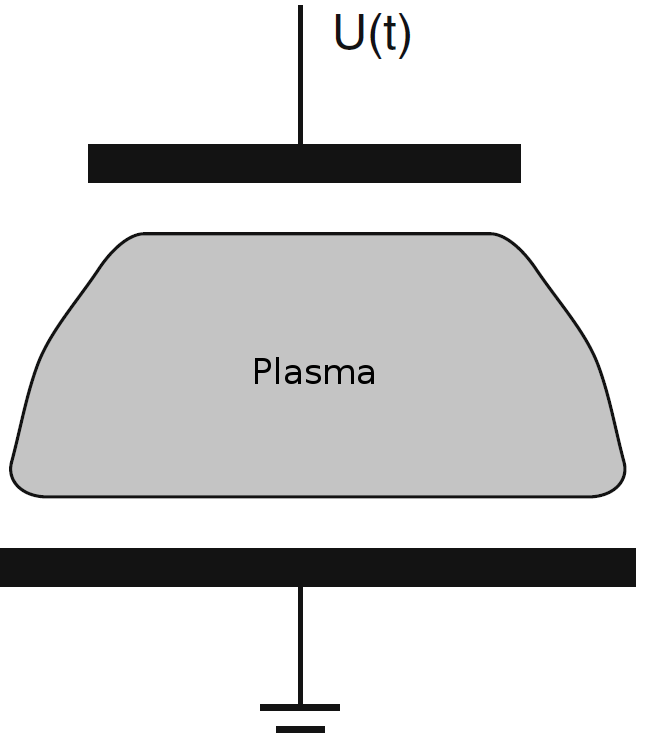
\includegraphics[width=0.3\textwidth,height=0.35\textwidth]{figures/circuitselfbias_1.png}
				\caption{%
				Schematic of an asymmetric discharge with one grounded and one driven electrode.%
				The rf signal is denoted with $U(t)$.}\label{fig:circuitselfbias_1}
			\end{wrapfigure}

      In the case of different electrode sizes, as seen in the scheme, the potential inside the spatially restricted area between wall and discharge can change drastically. This plasma sheath forms also between grounded parts of discharge containment or probes and plasma volume. This additional direct current offset is called \emph{self-bias} (see~\autoref{subsec:selfbias}). A dielectric displacement current between plasma sheath and volume accomodates as a result of the different time scales of particle movement (see~\autoref{subsec:displacementcurrent}). Especially, self-bias and displacement current play a key role in the following investigations, as a capacitive coupling between electrodes and power supply is difficult to model into a numerical kinetic simulation.\\
		In comparison to other low temperature, low pressure discharges  --- an example could be a dielectric hindered dc discharge at high voltages, with an electrode space gap of just a couple millimeters ---, radio frequency plasma are characterized by their unique transport process inside the sheath and heating mechanisms of charged species. 

		\subsection{Sheath physics and wall interaction}\label{subsec:sheathphysics}

		\subsection{Bohm criteria}\label{subsec:bohmcriteria}

    \subsection{Self bias voltage}\label{subsec:selfbias}

    \subsection{Dielectric displacement current}\label{subsec:displacementcurrent}

  \section{Negative ion physics}

    \subsection{Anion creation and distribution}

    \subsection{Dynamics and collisions}

  \section{Particle-In-Cell simulations with Monte Carlo-Colissions}

    \subsection{Principles}

    \subsection{2d3v PIC}

    \subsection{Monte Carlo-Collisions}

\chapter{Validation of Simulation by 1d comparison}

  \section{Axial density profiles}

  \section{Velocity and energy distributions}

  \section{Transition to 2d simulation}

\chapter{Simulation of capacitively coupled rf discharges}

  \section{Experimental setup}

  \section{Secondary ion emission}
  
  \section{Anion energy distributions in oxygen}

\chapter{Epilogue}

	\section{Local electrostratic field solver}

  \section{Diagnostics of current and charge}
  
  \section{Field calculation}

  \section{Comparison with Poisson-based solvers}

\chapter{Conclusion}

% ************************************************************************** %
	
% ************************************************************************** %
% APPENDICES
	\appendix % Cue to tell LaTeX that following "chapters" are Appendices
	% Include the appendices of the thesis as separate files
	% Uncomment the lines as you write the Appendices
	\chapter{Appendix}
%
% ************************************************************************** %
% PHYSICAL PROPERTIES
  \section{Physical Properties}
  \begin{longtable}{m{0.32\textwidth}m{0.32\textwidth}m{0.32\textwidth}}
    \toprule
    \bfseries quantity & \bfseries equation & \bfseries relevance \\%
    \toprule\midrule\endhead%
      Debye length &%
        $\begin{aligned}
          \lambda\ix{D,j}^2&=\frac{\varepsilon\ix{0}k\ix{B}T\ix{j}}{n\ix{j}e^2} \\
          \lambda\ix{D}^2&={\left(\lambda\ix{D,e}^{-2}+\lambda\ix{D,i}^{-2}\right)}^{-1}
        \end{aligned}$ &%
          distance around a charge, at which quasi-neutrality is satisfied, %
          $\lambda\ix{D}$ is the combined screening length from individual species \\ \midrule%
      plasma parameter &%
        $\begin{aligned}
          N\ix{D} = n\frac{4}{3}\pi\lambda\ix{D}^{3}
        \end{aligned}$ &%
        number of particles inside Debye sphere, if $N\ix{D} \gg 1$ an ionized gas %
        is considered a plasma (degree of ionization) \\ \midrule%
      plasma frequency &%
        $\begin{aligned}
          \omega\ix{p,j}^2=\frac{n\ix{j}e^2}{\varepsilon\ix{0}m\ix{j}}=%
          \frac{v\ix{th,j}}{\lambda\ix{D,j}}=\frac{1}{\tau\ix{j}}
        \end{aligned}$ &%
          upper limit for interaction with fields/forces or external excitations %
          inverse screening time \\ \midrule%
      thermal velocity &%
        $\begin{aligned}
          v\ix{th,j}^2=\frac{k\ix{B}T\ix{j}}{m\ix{j}}
        \end{aligned}$ &%
          mean velocity from kinetic theory of gases \\ \midrule%
      coulomb logarithm &%
        $\begin{aligned}
          &\ln\left(\Lambda\right) \\ \\
          &\Lambda=\frac{b\max}{b\min}= \\ \\
          &\lambda\ix{D}\cdot%
          \frac{4\pi\varepsilon\ix{0}\mu v\ix{th}^{2}}{e^{2}} 
        \end{aligned}$ &%
          dimensionless scale for transport processes inside discharge \newline
          fraction of probability for a cumulative $90^{\circ}$ scattering by many small %
          pertubation collisions and a single right angle scattering \\ \midrule%
      collision frequency &%
        $\begin{aligned}
          \nu\ix{j}=\frac{e^{4}n\ix{j}\ln\left(\Lambda\right)}%
          {8\sqrt{2m\ix{j}}\pi\varepsilon\ix{0}{\left(k\ix{B}T\ix{j}\right)}^{3/2}}
        \end{aligned}$ &%
          two body coulomb collision frequency inside species j \\ \midrule%
      particle distance \& \newline mean free path &%
        $\begin{aligned}
          &\overline{b}=\frac{\hbar}{m\ix{j}v\ix{th,j}} \\ \\
          &s\ix{mfp,j}=\frac{v\ix{th,j}}{\nu\ix{j,k}}
        \end{aligned}$ &%
          mean inter particle distance for species j \newline% 
          free flight between subsequent collisions of species j and k %
          with collision frequency $\nu\ix{j,k}$ \\ \midrule%
      speed of sound &%
        $\begin{aligned}
          c\ix{S}^{2}&=\frac{\gamma Zk\ix{B}T\ix{e}}{m\ix{i}} \\
          \gamma&=1+2/f=5/3
        \end{aligned}$ &%
        speed of longitudinal ion waves at electron pressure \newline%
        adiabatic coefficient with f, the kinetic degree of freedom\\ \midrule%
      Debye-Hückel potential &%
        $\begin{aligned}
          \Phi=\frac{Q}{4\pi\varepsilon|\vec{r}|}%
          \euler^{-\frac{|\vec{r}|}{\lambda\ix{D}}}
        \end{aligned}$ &%
        electrostatic potential of charge particle $Q$ at distance $|\vec{r}|$, \newline%
        equal to coulomb interaction with additional%
        shielding by charged particles \\ \midrule%
      drift velocity &
        $\begin{aligned}
          v\ix{d,j}=u\ix{j}=\frac{j\ix{j}}{n\ix{j}q}=\frac{m\sigma E}{\rho ef}
        \end{aligned}$ &%
        average velocity of a particle in a conductor with an electric field applied E, \newline%
        where $N$ is the number of free electrons per atom \\%
      electric mobility &
        $\begin{aligned}
          \mu\ix{j}=\frac{v\ix{d}}{E}
        \end{aligned}$ &%
        ability of charged particle of moving through an electric field \\%
    \midrule\bottomrule%
    \caption[Selection of physical properties of a low temperature ccrf discharge]{%
      Selection of physical properties of a low temperature ccrf discharge. The index $j$ denotes the %
      species, e.g.\@ electrons, ions. Used quantities can be found in the preface %
      in~\autoref{tabe:physicalconstants}.}\label{tabe:physicalquantities}
  \end{longtable}
% ************************************************************************** %
%   
		\clearpage
    \section[Energy Distributions from 2D PIC]%
            {Simulated Energy Distribution\\
            Functions from 2D PIC}\label{sec:appendix_results}
%
        \begin{center}
            \begin{figure}[!h]
                \centering
                \begin{subfigure}{0.49\textwidth}
									\includegraphics[height=0.3\textheight]%
                        {figures/results/2D/44332/e_dens.png}
                \end{subfigure}
                \begin{subfigure}{0.49\textwidth}
									\includegraphics[height=0.3\textheight]%
                        {figures/results/2D/44426/e_dens.png}
                \end{subfigure}
                %\caption[2D electron and ion density]{%
                %    Electron density from the two previously %
								%		described asymmetric 2D simulations.}
                %\label{fig:app_dens}
            %\end{figure}
						%\begin{figure}
								%\centering
                \begin{subfigure}{0.49\textwidth}
									\includegraphics[height=0.3\textheight]%
                        {figures/results/2D/44332/ni_dens.png}
                \end{subfigure}
                \begin{subfigure}{0.49\textwidth}
									\includegraphics[height=0.3\textheight]%
                        {figures/results/2D/44426/ni_dens.png}
                \end{subfigure}
								\newline
                %\caption[2D electron and ion density]{%
                %    Negative ion density from the two previously %
								%		described asymmetric 2D simulations.}
                %\label{fig:app_dens_ni}
            %\end{figure}
						%\begin{figure}[!b]
                %\centering
                \begin{subfigure}{0.49\textwidth}
									\includegraphics[height=0.22\textheight]%
                        {figures/results/2D/44332/e_distz.png}
                \end{subfigure}
                \begin{subfigure}{0.49\textwidth}
									\includegraphics[height=0.22\textheight]%
                        {figures/results/2D/44426/e_distz.png}
                \end{subfigure}
               	\caption[Electron and negative ion panel]{%
									\fett{Top}: electron density, \fett{Mid}: negative ion density, %
									\fett{Bottom}: axial compontent of electron EDF from a 2D simulation %
										of the two asymmetrical discharges discussed before-hand.}
                \label{fig:app_dens}
            \end{figure}
						\clearpage
            \begin{figure}
                \centering
                \begin{subfigure}{0.49\textwidth}
                    \includegraphics[width=1.0\textwidth]%
                        {figures/results/2D/44332/i_distz.png}
                \end{subfigure}
                \begin{subfigure}{0.49\textwidth}
                    \includegraphics[width=1.0\textwidth]%
                        {figures/results/2D/44426/i_distz.png}
                \end{subfigure}
                \caption[Axial ion EDF from 2D]{%
                    Axial compontent of ion EDF from a 2D simulation %
										of the two asymmetrical discharges discussed before-hand.}
                \label{fig:app_edf_i}
            \end{figure}
						\vfill
            \begin{figure}
                \centering
                \begin{subfigure}{0.49\textwidth}
                    \includegraphics[width=1.0\textwidth]%
                        {figures/results/2D/44332/ni_distz.png}
                \end{subfigure}
                \begin{subfigure}{0.49\textwidth}
                    \includegraphics[width=1.0\textwidth]%
                        {figures/results/2D/44426/ni_distz.png}
                \end{subfigure}
                \caption[Axial negative ion EDF from 2D]{%
                    Axial compontent of negative ion EDF from a 2D simulation %
										of the two asymmetrical discharges discussed before-hand.}
                \label{fig:app_edf_ni}
            \end{figure}
        \end{center}
%
		\clearpage
    \listoffigures % Prints the list of figures
	\listoftables % Prints the list of tables

% ************************************************************************** %

% ************************************************************************** %
% BIBLIOGRAPHY
	\printbibliography[heading=bibintoc]
% ************************************************************************** %

% END OF DOCUMENT
\end{document}  
